\chapter{Il mio lavoro - Titolo provvisorio}

\section{Introduzione}
%spiegare obiettivo
Il mio obiettivo è di creare un sistema di anomaly detection con struttura distribuita: nei router delle sedi periferiche raccolgo informazioni sul traffico e in un server posizionato fisicamente nella sede centrale lo analizzo e prendo decisioni sulle azioni da compiere. Per svolgere questo lavoro mi sono dovuto basare su alcuni software e sull'hardware aziendale con i relativi vantaggi e svantaggi rispetto ad una soluzione completamente ex-novo.
% spiegare come vengono gestiti i dati

\subsection{Gestione dei dati}

I dati vengono collezionati tramite un demone sui router (collectd), inviati al server (go-graphite) e visualizzati tramite una dashboard(graphana). Il tool di anomaly detection da me pensato si interfaccia direttamente con il database per la lettura dei dati e la scrittura dei risultati.
Qui in seguito approfondirò maggiormente il flusso della gestione dei dati.

\begin{figure}[]
    % todo: capire come gestire citazioni imsmagini a livello di copyright
    %  e capire come funzionano le label per richiamare le immagini
    \label{fig:mos}
    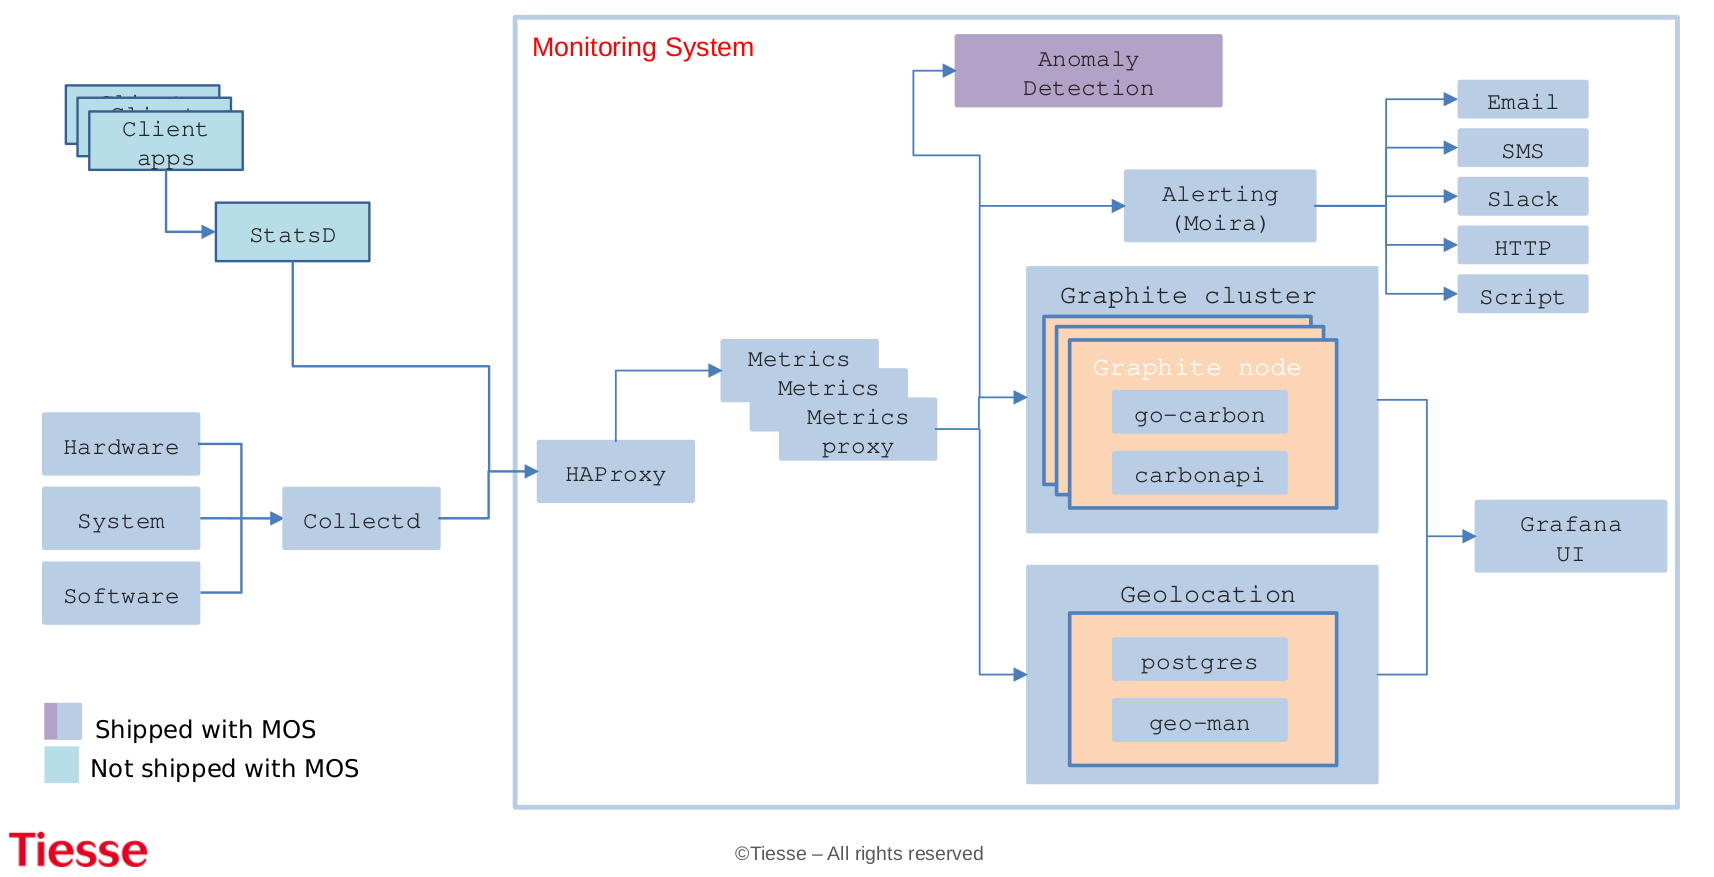
\includegraphics[width=\hsize]{images/my_work/tiesse_mos.png}
    \caption{Architettura di MOS (Monitor System di Tiesse)}
    \centering
\end{figure}

\paragraph{collectd} è un demone che raccoglie metriche di sistema e di applicazioni, trasferisce e salva dati di computer e dispositivi di rete. Collect ha una struttura modulare in cui è possibile abilitare centinaia di plugin per la raccolta di metriche di sistema dai casi più generali a quelli più specifici ed inoltre è possibile scrivere i propri plugin per integrarlo ulteriormente. I plugin da me usati sono ``write\_graphite'': plugin che permette di scrivere le metriche raccolte su un database graphite, ``conntrack'': plugin che permette di contare il numero di voci nella connection tracking table di Linux, ``interface'' : plugin che colleziona informazioni sul traffico su un'interfaccia, quindi pacchetti al secondo, bytes al secondo ed errori sull'interfaccia. 

Inoltre per avere ulteriori dati a disposizione ho scritto un plugin che si occupa di aggiungere delle metriche sul conteggio dei pacchetti non possibile con i plugin standard.

\paragraph{Il mio plugin di collect}

\paragraph{NDPI} è un software per il deep-packet inspection basato su OpenDPI
%http://luca.ntop.org/nDPI.pdf

\begin{itemize}
    \item carbon: è un service ad altre prestazioni che si occupa di ricevere le metriche con formato ``(timestamp, value)'' da salvare.
    \item whisper: un semplice database che salva sul filesystem le sequenze temporali di dati.
    \item graphite-web: è un'interfaccia utente e delle API le quali restituiscono i dati per renderizzare i grafici da visualizzare.
\end{itemize}
%todo: posso parlare della prima versione, dei problemi riscontrati e dell'utilizzo di ebpf al suo posto
\paragraph{graphite} è un software open source per il monitoraggio che può funzionare sia su hardware economico, che su un'infrastruttura cloud. Può essere usato per monitorare le performance di siti, applicazioni, server e nel caso di Tiesse è usato per monitorare informazioni sull'uso dei router, come per esempio il numero totale di router connessi, quelli raggiungibili, il throughput, l'uptime e la velocità della connessione xDSL.
L'obiettivo di graphite è il salvataggio di serie temporali di dati numerici e la successiva condivisione e visualizzazione.
Graphite è composto da tre parti (come si può vedere dalla figura ~\ref{fig:graphite}):

% https://www.aosabook.org/en/graphite.html
% https://graphiteapp.org/#gettingStarted
%todo: spiegare meglio come funzionano le carbon api

\begin{figure}[h]
    % todo: capire come gestire citazioni imsmagini a livello di copyright
    %  e capire come funzionano le label per richiamare le immagini
    \label{fig:graphite}
    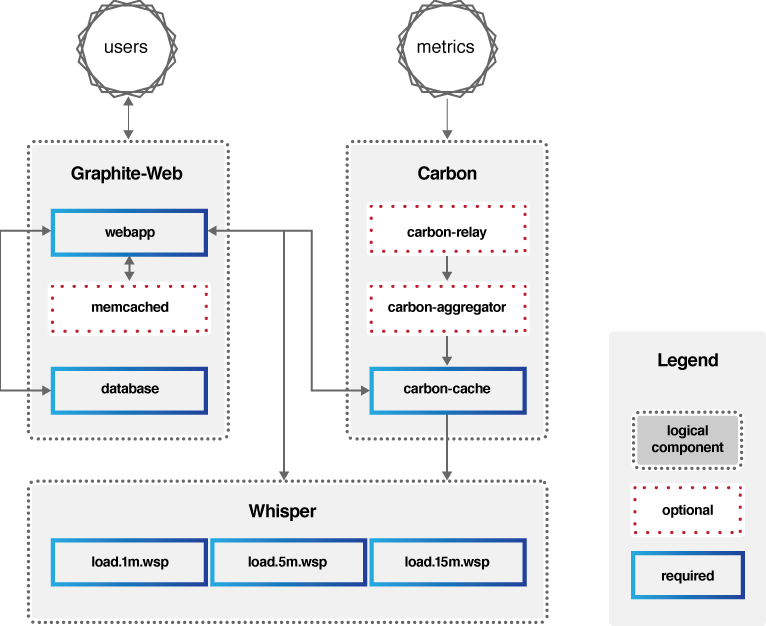
\includegraphics[width=\hsize]{images/my_work/graphite.png}
    \caption{Architettura di Graphite}
    \centering
\end{figure}

\paragraph{go-graphite} è un'implementazione in Golang di Graphite, rispetto a 
go-carbon più veloce vedi immagine
% https://github.com/go-graphite/go-carbon

carbonapi => subset di quelle di graphite, dalle 5 alle 10 volte più veloce di graphite-web

\begin{figure}[h]
    % todo: capire come gestire citazioni imsmagini a livello di copyright
    %  e capire come funzionano le label per richiamare le immagini
    \label{fig:graphana}
    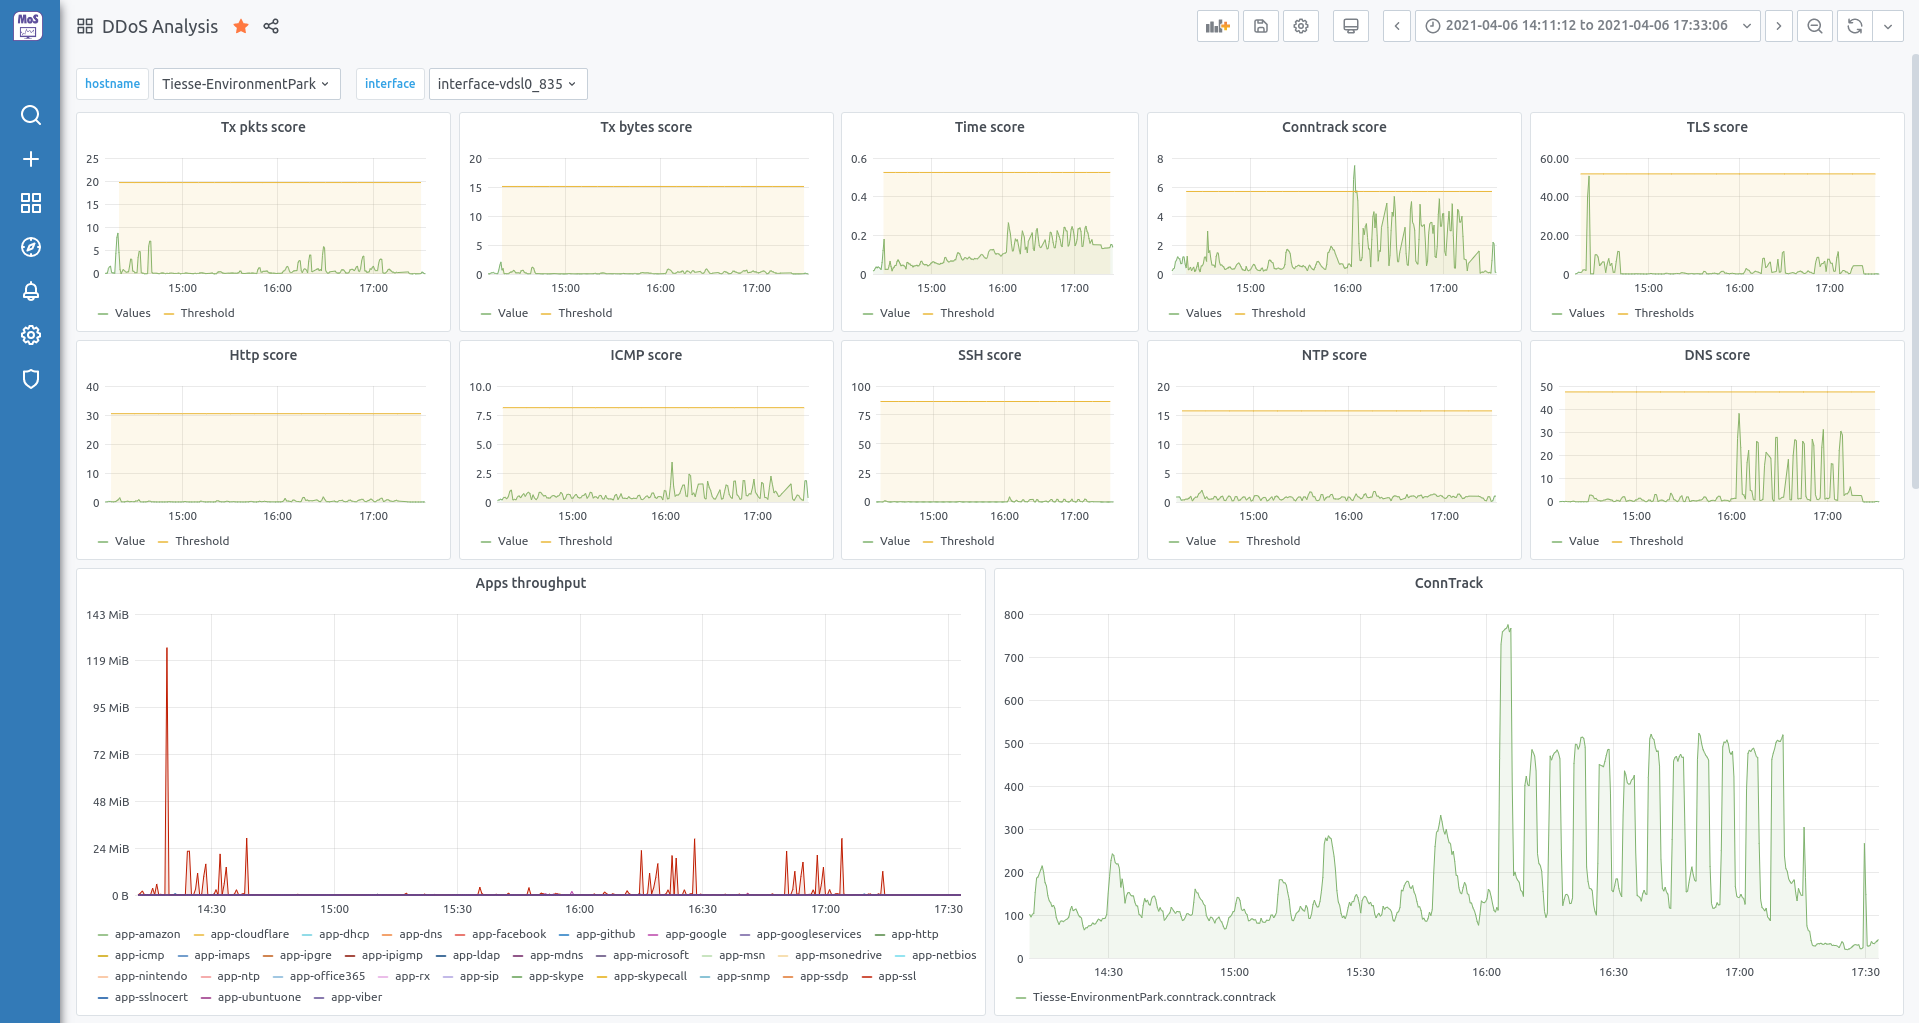
\includegraphics[width=\hsize]{images/my_work/grafana_dashboard.png}
    \caption{La mia dashboard su Grafana}
    \centering
\end{figure}

\paragraph{Grafana} è un software open source che permette la visualizzazione e la generazione delle metriche tramite una web application. Permette di creare dashboard dinamiche interrogando le api di graphite-web. Nel mio caso ho organizzato una dashboard in modo da visualizzare sia i dati provenienti dai router da analizzate, sia gli anomaly score calcolati dal software di anomaly-detection ~\ref{fig:graphana}.


%todo: come vengono mandati i dati di ndpi?
Riassumendo i dati provenienti dai plugin di collect, dal mio plugin e da NDPI vengono collezionati da collectd e inviati tramite il plugin write\_graphite al backend go-carbon, che si occupa di ricevere i dati e salvarli sul file system. Per la visualizzazione dei dati viene usato grafana, che permette di visualizzare i dati richiedendo i dati alle carbonapi e contemporaneamente il mio tool di anomaly detection richiede i dati per analizzarli, ogni volta che ottiene dei risultati li manda a go-carbon per salvarli nel database ~\ref{fig:mos}.
% todo: approfondire MOS
% todo: fare immagine con la gestione dei dati



\section{Selezione features}

La scelta delle feature da utilizzare dipende da quale obiettivo su vuole ottenere, il mio obiettivo primario in questa tesi è di rilevare gli attacchi DDoS in uscita verso la sede centrale, quindi basandomi sugli attacchi più famosi e frequenti ho delineato una lista di parametri da osservare. Questi parametri sono:
% todo: capire le unità di misura i dati sono ogni secondo o ogni 10
\begin{itemize}
    \item \emph{bytes trasmessi al secondo}:questa metrica è utile, abbinata ad altre, per la rilevazione di attacchi che mirano alla saturazione della banda.
    \item \emph{pacchetti trasmessi al secondo}: questa metrica ha uno scopo simile alla precedente oppure aiuta ad avere informazioni sugli attacchi di tipo flooding.
    \item \emph{numero di connessioni aperte} %todo: questa ha molti usi
    \item \emph{numero di pacchetti con flag syn}: questa metrica è molto utile per la rilevazione di syn flood o port scanning.
    \item \emph{tls throughput}: tutto il traffico inviato su un canale sicuro tls non può essere analizzato più nello specifico, quindi viene raggruppato in questa categoria.
    \item \emph{dns throughput}
    \item \emph{ssh throughput}
    \item \emph{icmp throughput}
    \item \emph{ora del giorno}: l'ora del giorno viene aggiunta per caratterizzare al meglio il traffico lungo la giornata.
\end{itemize}

Tutte le feature vengono poi derivate su un tempo di 10/30s, per avere dei "rate" confrontabili tra lavoro.

La scelta della features è nata da un compromesso tra i dati necessari per rilevare al meglio le anomalie, la riduzione dei dati da salvare sul server e di conseguenza l'uso di banda usata per il trasferimento. Inoltre un problema che ho dovuto tenere in considerazione è l'utilizzo di un acceleratore hardware nei router Tiesse, il quale permette un incremento della velocità di routing, ma non permette di analizzare nel kernel i pacchetti.
 %todo: approfondire meglio come funziona il fast path
 
 Per la raccolta dei dati sono stati usati dei plug

\section{Il mio tool}
\subsection{Struttura}
\subsection{Modello della rete}
\subsection{Train}
\subsection{Evaluate}


\section{Test sulle anomalie}
\subsection{Tool utilizzati}

Parlare come funzionano i tool che ho fatto

\subsection{Risultati}
